\documentclass[aspectratio=169]{beamer}

% --- Overleaf Compatibility & Encoding ---
\usepackage[utf8]{inputenc}
\usepackage[T1]{fontenc}
\usepackage{lmodern}


% --- Theme & Styling ---
\usetheme{Madrid}
\usecolortheme{seahorse}
\usefonttheme{professionalfonts}

\usepackage{graphicx}
\usepackage{booktabs}
\usepackage{tabularx} 
\usepackage{adjustbox} 
\usepackage{xcolor}
\usepackage{listings}
\usepackage{tikz}

% --- TikZ Libraries ---
\usetikzlibrary{shapes.geometric, arrows.meta, positioning, fit, backgrounds, decorations.pathreplacing}

% --- Custom Colors ---
\definecolor{agentblue}{RGB}{30, 80, 160}
\definecolor{agentgreen}{RGB}{34, 139, 34}
\definecolor{agentorange}{RGB}{210, 105, 30}
\definecolor{agentgray}{RGB}{100, 100, 100}
\definecolor{promptbg}{RGB}{245, 245, 250}
\definecolor{codebg}{RGB}{30, 30, 40}

% --- Listings Styles ---
\lstdefinestyle{prompt}{
  backgroundcolor=\color{promptbg},
  basicstyle=\ttfamily\fontsize{6}{7.5}\selectfont, 
  breaklines=true,
  breakatwhitespace=true,
  frame=single,
  rulecolor=\color{agentblue!40},
  framesep=3pt,
  xleftmargin=2pt,
  xrightmargin=2pt,
  aboveskip=2pt, 
  belowskip=2pt, 
  columns=fullflexible,
  keepspaces=true,
}

\lstdefinestyle{code}{
  backgroundcolor=\color{codebg},
  basicstyle=\ttfamily\fontsize{6}{7.5}\selectfont\color{white},
  breaklines=true,
  frame=none,
  xleftmargin=2pt,
  aboveskip=2pt,
  belowskip=2pt,
  columns=fullflexible,
  keepspaces=true,
}

% --- Beamer Template Adjustments ---
\setbeamertemplate{navigation symbols}{}
\setbeamertemplate{footline}[frame number]
\setbeamerfont{frametitle}{size=\large, series=\bfseries}
\setbeamertemplate{itemize items}[circle]

% --- Title Information ---
\title[GSU Virtual Academic Advisor]{\textbf{Virtual Academic Advisor}\\
  \large Agentic LLM System for GSU Graduation Analysis}
\author{INF473 Project Presentation}
\institute{Galatasaray University}
\date{May 9, 2026}

\begin{document}

% =================================================================
% TITLE & OUTLINE
% =================================================================
\begin{frame}
  \titlepage
\end{frame}

\begin{frame}{Outline}
  \tableofcontents
\end{frame}

% =================================================================
\section{Project Overview}
% =================================================================

\begin{frame}{What Is the Problem?}
  \begin{columns}[T]
    \begin{column}{0.54\textwidth}
      \begin{block}{Academic Advising Challenge}
        \begin{itemize}
          \item Transcripts are \textbf{unstructured text}
          \item Graduation requires \textbf{structured rule evaluation}
          \item Manual advising is slow and error-prone
        \end{itemize}
      \end{block}
      \vspace{0.2em}
      \begin{block}{Three Core Responsibilities}
        \begin{enumerate}
          \item Extract structured data via LLM
          \item Verify against GSU CE rules
          \item Generate human-readable reports
        \end{enumerate}
      \end{block}
    \end{column}
    \begin{column}{0.42\textwidth}
      \centering
      \vspace{1em}
      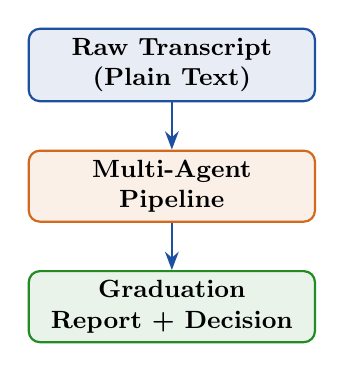
\begin{tikzpicture}[
        % FIX: Removed parameterized #1 to avoid Beamer errors
        basebox/.style={rectangle, rounded corners=4pt, text width=3.4cm, align=center, minimum height=0.8cm, font=\small\bfseries, thick},
        arr/.style={-Stealth, thick, color=agentblue}
      ]
        \node[basebox, draw=agentblue, fill=agentblue!10] (raw) {Raw Transcript\\(Plain Text)};
        \node[basebox, draw=agentorange, fill=agentorange!10, below=0.6cm of raw] (agent) {Multi-Agent\\Pipeline};
        \node[basebox, draw=agentgreen, fill=agentgreen!10, below=0.6cm of agent] (report) {Graduation\\Report + Decision};
        \draw[arr] (raw) -- (agent);
        \draw[arr] (agent) -- (report);
      \end{tikzpicture}
    \end{column}
  \end{columns}
\end{frame}

\begin{frame}{System at a Glance}
  \begin{columns}[T]
    \begin{column}{0.48\textwidth}
      \begin{block}{Tech Stack}
        \begin{itemize}
          \item \textbf{Backend:} FastAPI (Python)
          \item \textbf{LLM:} Groq API — \texttt{llama-3.3-70b}
          \item \textbf{Database:} SQLite via SQLAlchemy
          \item \textbf{Frontend:} React + Vite
          \item \textbf{Export:} jsPDF
        \end{itemize}
      \end{block}
      \begin{block}{Knowledge Base (\texttt{rules.py})}
        \begin{itemize}
          \item Min GPA: 2.00 / Min ECTS: 240
          \item 44 mandatory courses \& 6 electives
          \item 21 equivalency mappings
          \item Legacy curriculum transition rules
        \end{itemize}
      \end{block}
    \end{column}
    \begin{column}{0.48\textwidth}
      \begin{block}{API Endpoints}
        \footnotesize
        \renewcommand{\arraystretch}{1.2}
        \begin{tabularx}{\linewidth}{@{} l X @{}}
          \toprule
          \textbf{Method} & \textbf{Endpoint} \\
          \midrule
          POST & \texttt{/transcripts/upload} \\
          POST & \texttt{/analysis/analyze/\{id\}} \\
          GET  & \texttt{/analysis/\{id\}} \\
          GET  & \texttt{/analysis/history} \\
          DELETE & \texttt{/analysis/\{id\}} \\
          \bottomrule
        \end{tabularx}
      \end{block}
      \vspace{0.5em}
      \begin{alertblock}{Model Fallback Chain}
        \footnotesize \texttt{llama-3.3-70b} $\to$ \texttt{llama-3.1-8b} $\to$ \texttt{gemma2-9b}
      \end{alertblock}
    \end{column}
  \end{columns}
\end{frame}

% =================================================================
\section{Multi-Agent Architecture}
% =================================================================
\begin{frame}{Sequence Diagram}
  \begin{center}
    % The adjustbox ensures the image never overflows the slide boundaries
    \begin{adjustbox}{max height=0.75\textheight, max width=\linewidth}
    \IfFileExists{sequence_diagram2.png}{
        
\includegraphics{sequence_diagram2.png}
    }{
        % This placeholder shows up if the file isn't uploaded yet
        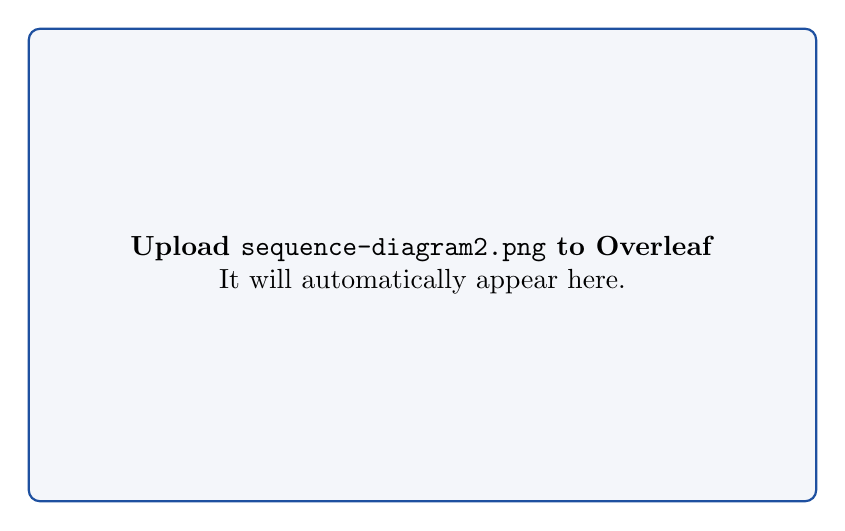
\begin{tikzpicture}
          \node[draw=agentblue, fill=agentblue!5, minimum width=10cm, minimum height=6cm, rounded corners=4pt, align=center, thick] 
          {\textbf{Upload \texttt{sequence-diagram2.png} to Overleaf}\\It will automatically appear here.};
        \end{tikzpicture}
    }
    \end{adjustbox}
  \end{center}
  
  \vspace{0.2em}
  \begin{center}
    \tiny\textit{Sequence diagram representing the full request-to-response flow}
  \end{center}
\end{frame}



\begin{frame}{10-Step Operational Pipeline}
  \begin{columns}[T]
    \begin{column}{0.48\textwidth}
      \begin{enumerate}
        \item \textbf{Input:} Paste/upload \texttt{.txt}
        \item \textbf{Validation:} Multi-transcript reject
        \item \textbf{Persistence:} SHA-256 deduplication
        \item \textbf{Parsing:} LLM extracts raw data
        \item \textbf{Evaluation:} 3 rule-based verifiers
      \end{enumerate}
    \end{column}
    \begin{column}{0.48\textwidth}
      \begin{enumerate}
        \setcounter{enumi}{5}
        \item \textbf{Cross-Check:} Agents verify logic
        \item \textbf{Master Decision:} Strict AND logic
        \item \textbf{Generation:} LLM + Database Tools
        \item \textbf{Review:} Critic agent polishes tone
        \item \textbf{Presentation:} UI render + PDF
      \end{enumerate}
    \end{column}
  \end{columns}
\end{frame}


% =================================================================
\section{Database \& Persistence}
% =================================================================

\begin{frame}{Database Schema \& Persistence}
  \begin{columns}[T]
    \begin{column}{0.48\textwidth}
      \begin{center}
        % Binds the image size to prevent slide overflow
        \begin{adjustbox}{max width=\linewidth, max height=0.75\textheight}
        \IfFileExists{db_schema.png}{
            
\includegraphics{db_schema.png}
        }{
            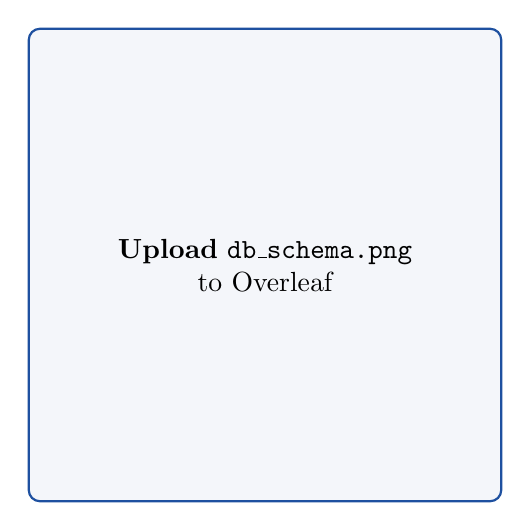
\begin{tikzpicture}
              \node[draw=agentblue, fill=agentblue!5, minimum width=6cm, minimum height=6cm, rounded corners=4pt, text width=5cm, align=center, thick] 
              {\textbf{Upload \texttt{db\_schema.png}}\\to Overleaf};
            \end{tikzpicture}
        }
        \end{adjustbox}
      \end{center}
    \end{column}
    \begin{column}{0.48\textwidth}
      \begin{block}{Core Tables}
        \footnotesize % Reduced from \small to prevent bottom overflow
        \begin{itemize}
          \setlength{\itemsep}{0.3em} % Tightens the space between bullet points
          \item \textbf{students}: Identity mapping (\texttt{student\_number}, name).
          \item \textbf{transcripts}: Stores raw text and \texttt{text\_hash} (SHA-256) for deduplication.
          \item \textbf{analysis\_results}: Caches GPA, ECTS, agent verdicts JSON, and final \texttt{report\_text}.
        \end{itemize}
      \end{block}
      
      \vspace{-0.2em} % Reduces the gap between the two blocks
      
      \begin{alertblock}{Design Highlights}
        \footnotesize % Reduced from \small
        \begin{itemize}
          \setlength{\itemsep}{0.3em}
          \item \textbf{Deduplication:} SHA-256 hashing prevents redundant (and costly) LLM API calls for identical transcripts.
          \item \textbf{Agentic Memory:} Provides the historical context queried by the \texttt{check\_history} tool.
        \end{itemize}
      \end{alertblock}
    \end{column}
  \end{columns}
\end{frame}
% =================================================================
\section{Agent Roles}
% =================================================================

\begin{frame}{Agent Roster}
  \small
  \renewcommand{\arraystretch}{1.3}
  \begin{tabularx}{\linewidth}{@{} p{3.2cm} p{2.2cm} X @{}}
    \toprule
    \textbf{Agent Name} & \textbf{Type} & \textbf{Responsibility} \\
    \midrule
    \textbf{TranscriptParser} & \textcolor{agentblue}{\bfseries LLM} & Extracts identity, GPA, and all courses (incl. failed) from raw text. \\
    \textbf{CourseVerifier} & \textcolor{agentgreen}{\bfseries Rule-based} & Checks mandatory completion, applies code normalizations \& equivalencies. \\
    \textbf{ECTSVerifier} & \textcolor{agentgreen}{\bfseries Rule-based} & Filters passed courses, sums ECTS, and verifies $\geq$ 240 threshold. \\
    \textbf{Requirements} & \textcolor{agentgreen}{\bfseries Rule-based} & Evaluates GPA, language goals, elective groups, and legacy transitions. \\
    \textbf{MasterAgent} & \textcolor{agentorange}{\bfseries Orchestrator} & Aggregates independent verdicts and triggers the final report workflow. \\
    \textbf{MasterReport} & \textcolor{agentblue}{\bfseries LLM + Tool} & Generates human-readable advisor report; queries historical DB. \\
    \textbf{ReportCritic} & \textcolor{agentblue}{\bfseries LLM} & Reviews draft, scrubs machine-like wording, ensures academic tone. \\
    \bottomrule
  \end{tabularx}
\end{frame}

\begin{frame}{Rule-Based Verifiers — Deep Dive}
  \begin{columns}[T]
    \begin{column}{0.32\textwidth}
      \begin{block}{CourseVerifier}
        \scriptsize
        \begin{itemize}
          \item Strip section suffixes (\texttt{-A}/\texttt{-B})
          \item Match against 44 codes
          \item Apply 21 equivalencies
          \item Output: completed vs. missing
        \end{itemize}
      \end{block}
    \end{column}
    \begin{column}{0.32\textwidth}
      \begin{block}{ECTSVerifier}
        \scriptsize
        \begin{itemize}
          \item Filter fails (\texttt{FF, DZ, F})
          \item Sum passed ECTS
          \item Enforce $\geq$ 240 check
          \item Output: surplus or deficit
        \end{itemize}
      \end{block}
    \end{column}
    \begin{column}{0.32\textwidth}
      \begin{block}{RequirementsAgent}
        \scriptsize
        \begin{itemize}
          \item Enforce GPA $\geq$ 2.00
          \item Language: 12 ECTS or B2
          \item 6 elective group rules
          \item Output: structural issues
        \end{itemize}
      \end{block}
    \end{column}
  \end{columns}
  \vspace{0.8em}
  \begin{alertblock}{Cross-Examination Process}
    \small Each verifier runs \texttt{cross\_examine()} on peer outputs to find correlations. Example: CourseVerifier flags an ECTS deficit as explicitly tied to \textit{"failed mandatory core classes."}
  \end{alertblock}
\end{frame}

\begin{frame}[fragile]{Data Flow \& Decision Logic}
  \begin{columns}[T]
    \begin{column}{0.48\textwidth}
      \begin{block}{Verdict Schema (Pydantic)}
        \begin{lstlisting}[style=code]
class AgentVerdict(BaseModel):
    agent: str
    verdict: str       # "pass" | "fail"
    statement: str
    issues: list[str]
    details: dict
        \end{lstlisting}
      \end{block}
      \begin{block}{Master Decision Rule}
        \centering
        \vspace{0.2em}
        \texttt{graduated = ALL verdicts == "pass"}
        \vspace{0.2em}\\
        \footnotesize Strict AND operator prevents false positives.
      \end{block}
    \end{column}
    \begin{column}{0.48\textwidth}
      \begin{block}{Frontend Payload Contents}
        \small The final JSON to the UI includes:
        \begin{itemize}
          \item Individual agent \texttt{verdicts}
          \item Consolidated \texttt{issues} list
          \item \texttt{completed\_courses} array
          \item \texttt{missing\_courses} array
          \item \texttt{report\_text} (LLM-generated)
          \item \texttt{tool\_logs} (DB comparisons)
        \end{itemize}
      \end{block}
    \end{column}
  \end{columns}
\end{frame}

% =================================================================
\section{Prompts \& Logic}
% =================================================================

\begin{frame}[fragile]{Prompt Engineering: Transcript Parser}
  \begin{block}{\texttt{PARSE\_SYSTEM\_PROMPT} (Excerpt)}
    \begin{lstlisting}[style=prompt]
You are a university transcript parsing expert. Extract ALL courses from a GSU transcript.
Column mapping: Kodu -> code (keep -A/-B), Ders Adi -> name, Notu -> grade, AKTS -> ects (int)
GPA extraction: Use the LAST "Genel" row, second column.

Return ONLY valid JSON:
{
  "student_number": string, "gpa": number, 
  "courses": [{"code": string, "name": string, "grade": string, "ects": integer}]
}
Rules: Include ALL courses (even F, FF, DZ). Return raw JSON only, no markdown.
    \end{lstlisting}
  \end{block}
  \vspace{-0.5em}
  \begin{columns}[T]
    \begin{column}{0.48\textwidth}
      \textbf{Design Choices:}
      \begin{itemize}
        \scriptsize
        \item Explicit column mapping prevents hallucinations.
        \item \textbf{Deterministic GPA check:} Regex guarantees the math overrides LLM extraction if needed.
      \end{itemize}
    \end{column}
    \begin{column}{0.48\textwidth}
      \textbf{Exclusion Directives:}
      \begin{itemize}
        \scriptsize
        \item Skips semester header rows safely.
        \item Discards "Kredi" in favor of "AKTS".
      \end{itemize}
    \end{column}
  \end{columns}
\end{frame}

\begin{frame}[fragile]{Report Generation \& Polish (Two-Stage)}
  \begin{columns}[T]
    \begin{column}{0.54\textwidth}
      \begin{block}{1. \texttt{REPORT\_SYSTEM\_PROMPT}}
        \begin{lstlisting}[style=prompt]
Write a 2-3 sentence graduation status report.
Base your report strictly on the provided analysis.
Do NOT expose internal machine values, field names, enums, or raw booleans (e.g. true, false, pass).
Interpret the master decision semantically.
        \end{lstlisting}
      \end{block}
      \begin{block}{2. \texttt{REVIEW\_SYSTEM\_PROMPT}}
        \begin{lstlisting}[style=prompt]
You are the ReportCriticAgent.
Review the draft report. Preserve the factual decision and key blockers. Keep it formal.
Rewrite to scrub any leaked internal variables.
        \end{lstlisting}
      \end{block}
    \end{column}
    \begin{column}{0.44\textwidth}
      \begin{block}{Why Two Stages?}
        \centering
        \begin{adjustbox}{max height=0.55\textheight, max width=\linewidth}
        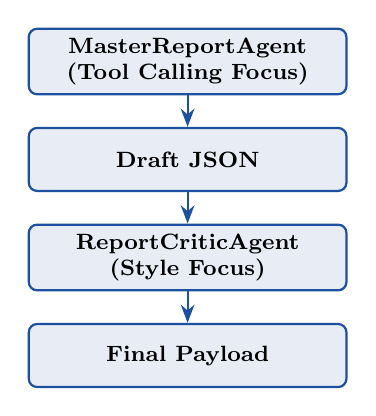
\begin{tikzpicture}[
          node distance=0.4cm,
          % FIX: Removed parameterized #1
          basebox/.style={rectangle, rounded corners=3pt, text width=3.8cm, align=center, font=\footnotesize\bfseries, minimum height=0.8cm, thick},
          arr/.style={-Stealth, thick, color=agentblue}
        ]
          \node[basebox, draw=agentblue, fill=agentblue!10] (rep) {MasterReportAgent\\(Tool Calling Focus)};
          \node[basebox, draw=agentblue, fill=agentblue!10, below=of rep] (draft) {Draft JSON};
          \node[basebox, draw=agentblue, fill=agentblue!10, below=of draft] (critic) {ReportCriticAgent\\(Style Focus)};
          \node[basebox, draw=agentblue, fill=agentblue!10, below=of critic] (final) {Final Payload};
          
          \draw[arr] (rep) -- (draft);
          \draw[arr] (draft) -- (critic);
          \draw[arr] (critic) -- (final);
        \end{tikzpicture}
        \end{adjustbox}
      \end{block}
      \vspace{0.2em}
      \scriptsize Tool execution often pollutes the LLM's context window. The Critic ensures the final frontend text is clean and academic.
    \end{column}
  \end{columns}
\end{frame}

% =================================================================
\section{Tool Calling \& Memory}
% =================================================================

\begin{frame}[fragile]{Tool Calling: \texttt{check\_student\_history}}
  \begin{columns}[T]
    \begin{column}{0.48\textwidth}
      \begin{block}{Tool Definition}
        \begin{lstlisting}[style=code]
{
  "name": "check_history",
  "description": "Queries SQLite for student's past GPA and graduation status.",
  "parameters": {
    "student_number": {"type": "string"}
  }
}
        \end{lstlisting}
      \end{block}
      \begin{alertblock}{Frontend Transparency}
        \scriptsize UI renders the tool log explicitly:\\
        \textit{"GPA increased from 2.31 to 2.49. Student now meets graduation requirements."}
      \end{alertblock}
    \end{column}
    \begin{column}{0.48\textwidth}
      \begin{block}{Tool-Calling Execution Flow}
        \centering
        \begin{adjustbox}{max height=0.65\textheight, max width=\linewidth}
        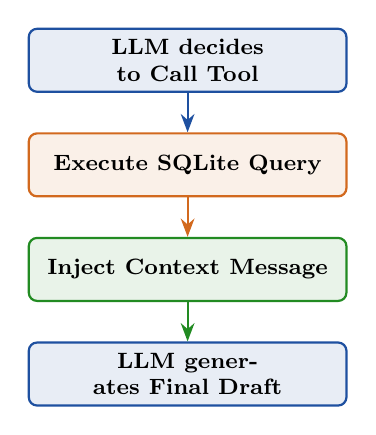
\begin{tikzpicture}[
          node distance=0.5cm,
          % FIX: Removed parameterized #1 
          basebox/.style={rectangle, rounded corners=3pt, text width=3.8cm, align=center, font=\footnotesize\bfseries, minimum height=0.8cm, thick},
          arr/.style={-Stealth, thick}
        ]
          \node[basebox, draw=agentblue, fill=agentblue!10] (llm1) {LLM decides\\to Call Tool};
          \node[basebox, draw=agentorange, fill=agentorange!10, below=of llm1] (tool) {Execute SQLite Query};
          \node[basebox, draw=agentgreen, fill=agentgreen!10, below=of tool] (res) {Inject Context Message};
          \node[basebox, draw=agentblue, fill=agentblue!10, below=of res] (llm2) {LLM generates Final Draft};
          
          \draw[arr, color=agentblue] (llm1) -- (tool);
          \draw[arr, color=agentorange] (tool) -- (res);
          \draw[arr, color=agentgreen] (res) -- (llm2);
        \end{tikzpicture}
        \end{adjustbox}
      \end{block}
    \end{column}
  \end{columns}
\end{frame}

% =================================================================
% =================================================================
\section{Frontend Interface}
% =================================================================

\begin{frame}{UI Interface Overview}
  \begin{columns} % <-- This MUST be here to use a column
    \begin{column}{0.6\textwidth} 
      \begin{block}{Interactive Result Features}
        \begin{itemize}
          \item \textbf{Status Banner:} Instant visual pass/fail indicator.
          \item \textbf{Advisor Summary:} LLM generated text block.
          \item \textbf{Metric Cards:} GPA and ECTS totals.
          \item \textbf{Expandable Verdicts:} Deep dive into exactly what each Agent evaluated.
          \item \textbf{Export:} Native \texttt{jsPDF} conversion for saving reports.
        \end{itemize}
      \end{block}
      \vspace{0.5em}
      \footnotesize \textbf{Database History Tab:} Allows users to browse past hashes, ensuring persistence.
    \end{column}
  \end{columns}
\end{frame}
% =================================================================
\section{Conclusion}
% =================================================================

\begin{frame}{Testing \& Conclusion}
  \begin{columns}[T]
    \begin{column}{0.48\textwidth}
      \begin{block}{Validation via 20-Scenario Suite}
        We tested the pipeline against complex edge cases including:
        \begin{itemize}
          \scriptsize
          \item Legacy curriculum baselines
          \item Equivalent course replacements
          \item Failed mandatory subjects mapped to new electives
          \item Missing language benchmarks
        \end{itemize}
      \end{block}
    \end{column}
    \begin{column}{0.48\textwidth}
      \begin{block}{Future Implementations}
        \begin{itemize}
          \scriptsize
          \item \textbf{OCR Integration:} Allow PDF/Image parsing directly.
          \item \textbf{Prerequisite Chain Check:} Verify sequential course integrity.
          \item \textbf{Scale to Multi-Department:} Parameterize rules via DB rather than static python files.
        \end{itemize}
      \end{block}
    \end{column}
  \end{columns}
  \vspace{0.8em}
  \begin{block}{Architectural Insight}
    \small Pragmatic separation of concerns: \textbf{LLMs} handle unstructured text, while strict \textbf{Rule-based scripts} lock down the high-stakes graduation logic.
  \end{block}
\end{frame}

\begin{frame}{}
  \begin{center}
    \vspace{2em}
    {\Huge\bfseries Thank You}\\[1em]
    {\large Questions?}\\[2em]
    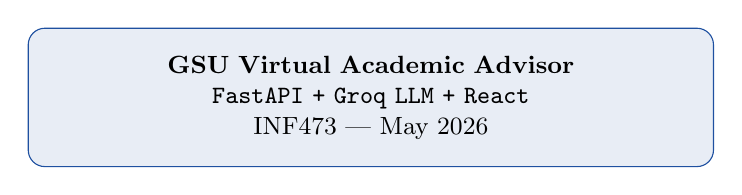
\begin{tikzpicture}
      \node[rectangle, rounded corners=6pt, draw=agentblue, fill=agentblue!10,
            text width=8cm, align=center, font=\small, inner sep=10pt] {
        \textbf{GSU Virtual Academic Advisor}\\
        \texttt{FastAPI + Groq LLM + React}\\
        INF473 — May 2026
      };
    \end{tikzpicture}
  \end{center}
\end{frame}

\end{document}